\section{Tests}\label{sec:tests}
Funktionelle tests, altså tests der påviser at funktionaliteten af klienten virker som ønsket, 
anvendes til at overbevise teamet om, at systemet fungerer som det skal. 
Denne slags test kaldes for ”Black-Box testing" og kan udføres af teamet, 
et dedikeret test-team eller i nogle tilfælde kunden som en del af en ”Acceptance-Test”. 
På den anden side befinder ”White-Box testing" sig, hvilket påviser interne elementer i selve koden. \\

\textbf{Test af klienten} \\
Gruppen har i projektperioden testet diverse funktionaliteter på klientsiden, 
men også i selve koden. I backenden er der anvendt noget der hedder NUnit til testing af koden, 
hvori nogle datasæt er opsat til at teste kald til systemets API.\\

\begin{figure}[H]
    \centering
    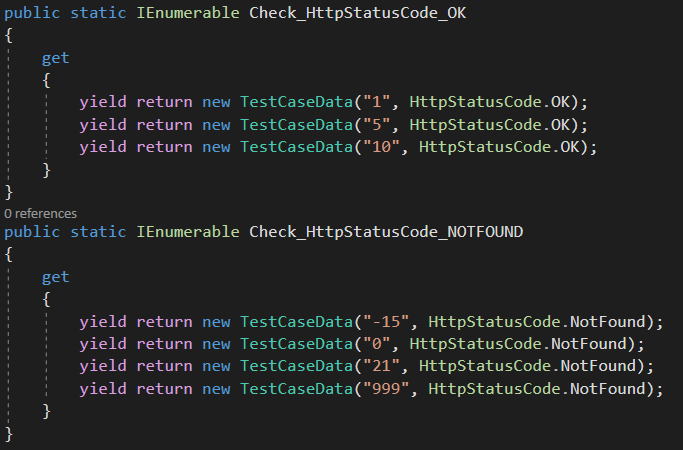
\includegraphics[width=0.8\textwidth]{figures/testmoviedata.PNG}
    \caption{Test data til test af Movies}
    \label{fig:testdata}
\end{figure}

I Figur \ref{fig:testdata} ses en række test data til test af movies i databasen. Ved "Check\_HttpStatusCode\_OK" findes det korrekte data,
som eksisterer i databasen. Ved "Check\_HttpStatusCode\_NotFound" findes værdier, som ikke eksisterer, og derfor vil give
en fejl besked. \\

I metoden på figur \ref{fig:testeks}, bliver data fra "Check\_HttpStatusCode\_OK" indsat i parameterne
og udført én efter én. Der testes altså her for eksisterende film i databasen. 

\begin{figure}[H]
    \centering
    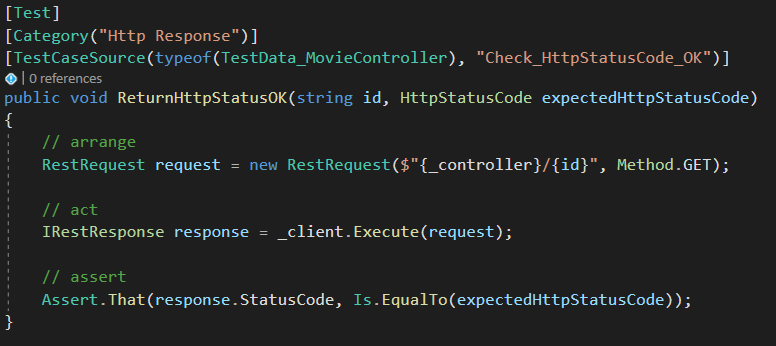
\includegraphics[width=0.8\textwidth]{figures/testmoviestatusok.PNG}
    \caption{Test af eksiterende data}
    \label{fig:testeks}
\end{figure}

I metoden på figur \ref{fig:testeks2}, bliver data fra "Check\_HttpStatusCode\_NotFound" indsat i parameterne
og udført én efter én. Der testes altså her for ikke eksiterende film i databasen. Dette skal selvfølgelig
give en fejlbesked.  

\begin{figure}[H]
    \centering
    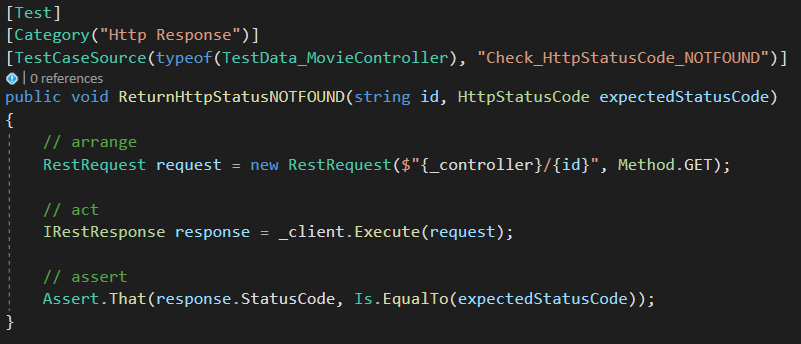
\includegraphics[width=0.8\textwidth]{figures/testmoviestatusnotfound.PNG}
    \caption{Test af fejl data}
    \label{fig:testeks2}
\end{figure}

Gruppen ser en fordel i at kunne genanvende en metode, 
frem for at skulle skrive en metode for hver enkelt test-case. 
Det giver et overblik og gør det betydeligt nemmere at ændre i data uden at skrive nye metoder eller fjerne dem.\\

\begin{figure}[H]
    \centering
    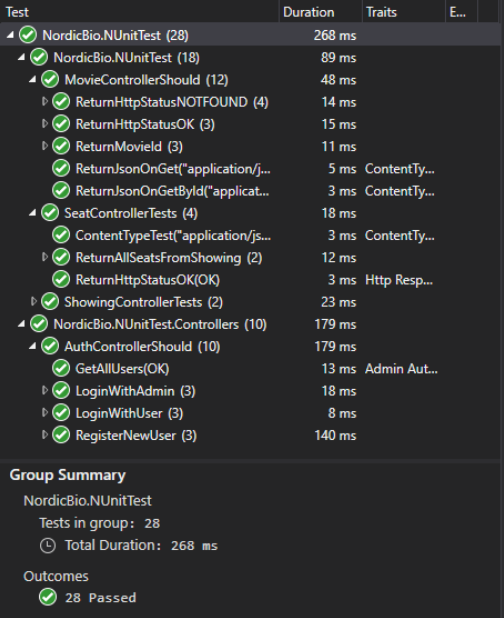
\includegraphics[width=0.6\textwidth]{figures/AllTests.png}
    \caption{Overblik af alle systemets tests}
    \label{fig:alltests}
\end{figure}


Systemet bliver testet gennem 28 forskellige tests, der kan ses på Figur \ref{fig:alltests}, hvilket ikke er en ret stor testdækning. 
Gruppen har fokuseret på at udvise forståelse for tests og testet, ud fra gruppens syn de vigtigste funktionaliteter.    